\documentclass[conference]{IEEEtran}
\IEEEoverridecommandlockouts

% ── Packages ─────────────────────────────────────────────────
\usepackage{cite}
\usepackage{amsmath,amssymb,amsfonts}
\usepackage{algorithm}
\usepackage{algpseudocode}
\usepackage{graphicx}
\usepackage{textcomp}
\usepackage{xcolor}
\usepackage{booktabs}
\usepackage{multirow}
\usepackage{url}
\usepackage{hyperref}
\usepackage{float}
\usepackage{array}
\usepackage{tabularx}
\usepackage{subcaption}
\graphicspath{{../../results/phase3/}}

\hypersetup{
    colorlinks=true,
    linkcolor=blue,
    citecolor=blue,
    urlcolor=blue
}

\def\BibTeX{{\rm B\kern-.05em{\sc i\kern-.025em b}\kern-.08em
    T\kern-.1667em\lower.7ex\hbox{E}\kern-.125emX}}

% ─────────────────────────────────────────────────────────────
\begin{document}

\title{AgriVision Phase 3:\\
A Hybrid BiLSTM--SVR Model for Crop Yield Prediction}

\author{
\IEEEauthorblockN{AgriVision Project}
\IEEEauthorblockA{
\textit{Satellite-Based Precision Agriculture}\\
Dataset: FAO Crop Yield (Kaggle) \quad
101 Countries $\cdot$ 10 Crops $\cdot$ 1990--2013
}
}

\maketitle

% ── Abstract ─────────────────────────────────────────────────
\begin{abstract}
This report describes Phase 3 of the AgriVision project: a hybrid model that combines the deep-learning network from Phase 2 with the support vector regressor from Phase 1. The idea is simple. Phase 1 (SVR) is good at fitting smooth boundaries on tabular data but cannot use the history of climate over multiple years. Phase 2 (BiLSTM with attention) reads a 5-year window of weather and learns useful patterns from it, but its final layer is just a single linear projection that can be sensitive to outliers. Phase 3 keeps the strengths of both: we freeze the trained BiLSTM, use it as a feature extractor to convert each 5-year sequence into a 64-dimensional vector, and then train an SVR to map those vectors to crop yield. On the held-out test set the hybrid achieves $R^{2}=0.951$ and $\text{RMSE}=1.90$~t/ha, the best result of the whole project. We also run an ablation study with four model variants and find that the BiLSTM embeddings alone (without the original 8 hand-crafted features) are enough — adding them back is slightly worse because the BiLSTM had already absorbed them through its skip connection.
\end{abstract}

\begin{IEEEkeywords}
crop yield prediction, hybrid model, support vector regression, BiLSTM, attention, ablation study, transfer learning
\end{IEEEkeywords}

% ─────────────────────────────────────────────────────────────
\section{Introduction}
\label{sec:intro}

\subsection{The Problem in Plain Terms}
Given a (country, crop, year) record together with rainfall, temperature, and pesticide use, predict the crop yield in tonnes per hectare. The same value of rainfall can produce very different yields depending on the crop's history: a single dry year hurts less than three dry years in a row. So a good model needs to use both \emph{this year's} numbers and the \emph{recent past}.

\subsection{Story of the Three Phases}
The project was built up in three steps, each fixing a weakness of the previous one.

\begin{itemize}
    \item \textbf{Phase 1 — Classical SVR.} We engineered eight static features (country code, crop code, rainfall, temperature, pesticides, log-pesticides, rainfall/temperature ratio, heat-stress index) and fit a tuned RBF Support Vector Regressor. The model is robust and easy to tune but only sees one year at a time. Final test $R^{2} = 0.782$.
    \item \textbf{Phase 2 — BiLSTM with Attention.} For every record we built a 5-year lookback window of climate data and fed it to a Bidirectional LSTM. An attention layer learns which year in the window matters most. A skip connection sends the static (country, crop) information straight to the layer just before the output, so the LSTM can focus on climate patterns. Test $R^{2} = 0.929$.
    \item \textbf{Phase 3 — Hybrid (this report).} The BiLSTM is now ``frozen.'' Instead of using its final prediction we open it up, take out the 64-dimensional vector that lives just before the output layer, and use that as a feature for an SVR. The SVR is good at producing smooth, robust predictions on top of these rich features. Test $R^{2} = 0.951$.
\end{itemize}

In short: \emph{Phase 2 learns what to look at; Phase 3 reuses that knowledge with a more robust regressor.}

\subsection{What This Report Answers}
\begin{enumerate}
    \item Does feeding BiLSTM features to an SVR improve over either model alone?
    \item Should we also add the original 8 features back, or are the BiLSTM features sufficient?
    \item Where does the improvement come from? An ablation study answers this directly.
\end{enumerate}

% ─────────────────────────────────────────────────────────────
\section{Related Work}
\label{sec:lit}

Crop yield modelling has gone through the same transition this project mirrors. Kaul \emph{et al.}~\cite{kaul2005} and Jeong \emph{et al.}~\cite{jeong2016} used SVR and Random Forests on tabular features, which work well but cannot capture history. Khaki and Wang~\cite{khaki2019} introduced LSTMs for corn yield, showing that multi-year sequences improve accuracy. Feng \emph{et al.}~\cite{feng2019} found that a 5-year window captures most of the useful temporal signal — this is the lookback length we use. Bahdanau \emph{et al.}~\cite{bahdanau2015} introduced the attention mechanism we adapt to weight the years in the lookback.

Outside agriculture, ``deep features into a classical model'' is a well-known recipe~\cite{lecun2015}: train a deep network, drop its final layer, and use its internal representation as input to a simpler classifier. Phase 3 is this recipe applied to crop yield prediction.

% ─────────────────────────────────────────────────────────────
\section{Method}
\label{sec:methodology}

\subsection{High-Level Picture}
The full pipeline is shown in Fig.~\ref{fig:overview}. There are three stages.
\begin{enumerate}
    \item \textbf{Reuse Phase 2.} We load the trained BiLSTM. Its weights stay frozen.
    \item \textbf{Extract embeddings.} For every record in the dataset, we run the BiLSTM forward and grab the 64-dim vector from the layer just before its final output. We call this vector $\mathbf{e}_i$.
    \item \textbf{Train SVR.} We train a tuned RBF SVR to map $\mathbf{e}_i$ (and optionally also the 8 original static features) to per-crop normalized yield, then invert the normalization to report errors in t/ha.
\end{enumerate}

\subsection{What Is the 64-Dim Embedding?}
Inside the BiLSTM, after attention pooling and two fully-connected layers, there is a 64-dim representation that summarises everything the network has learned about a sequence. The next operation is a single linear layer that maps this 64-dim vector to the predicted yield. We tap the 64-dim vector before the final layer:
\begin{equation}
\mathbf{e}_i \;=\; \underbrace{\operatorname{ReLU}\!\big(\operatorname{BN}(\mathbf{W}_2 \mathbf{h}_i)\big)}_{\text{climate context}} \;+\; \underbrace{\mathbf{W}_{\text{skip}}\,\mathbf{s}_i}_{\text{country/crop info}}
\end{equation}
This is important: the embedding $\mathbf{e}_i$ already mixes the temporal climate context with the static country/crop signal, because of the skip connection from Phase 2. We will see why this matters in Section~\ref{sec:results}.

To extract $\mathbf{e}_i$ in practice we use a PyTorch \texttt{forward\_hook} on the final linear layer (\texttt{fc\_out}). The hook records whatever vector arrives at that layer's input, which is exactly $\mathbf{e}_i$. The procedure is shown in Algorithm~\ref{alg:extract}.

\begin{algorithm}[H]
\caption{Extract BiLSTM Embeddings for the Whole Dataset}\label{alg:extract}
\begin{algorithmic}[1]
\Require trained BiLSTM $\mathcal{M}$, full dataset $\mathcal{D}$, sequence/static scalers from Phase 2
\Ensure embedding matrix $\mathbf{E}$ with one row per record
\State Put $\mathcal{M}$ in evaluation mode (disables dropout)
\State Attach a forward hook on the last linear layer that records its input
\For{each batch (sequence $\mathbf{X}$, static $\mathbf{s}$) in $\mathcal{D}$}
    \State Apply Phase-2 scalers to $\mathbf{X}$ and $\mathbf{s}$
    \State Run $\mathcal{M}(\mathbf{X}, \mathbf{s})$ — the hook captures $\mathbf{e}$
    \State Append $\mathbf{e}$ to $\mathbf{E}$
\EndFor
\State Remove the hook
\State \Return $\mathbf{E}$
\end{algorithmic}
\end{algorithm}

\subsection{Building the Hybrid Feature Vector}
For each record $i$ we now have two things:
\begin{itemize}
    \item the 64-dim BiLSTM embedding $\mathbf{e}_i$,
    \item the 8 static features $\mathbf{s}^{*}_i$ from Phase 1 (country code, crop code, rainfall, temperature, pesticides, log-pesticides, rainfall/(temp$+1$), heat-stress index).
\end{itemize}
We stack them to get a 72-dim hybrid vector $\mathbf{z}_i = [\mathbf{s}^{*}_i \,\|\, \mathbf{e}_i]$. This is what the hybrid SVR consumes.

\subsection{Per-Crop Target Normalization}
Different crops have very different typical yields: cassava averages around 14~t/ha, soybeans around 1.7~t/ha. If we trained directly on raw yield, the SVR would essentially be predicting the crop label. To prevent this we normalize the target per crop:
\begin{equation}
\tilde{y}_i = \frac{y_i - \mu_{c(i)}}{\sigma_{c(i)}},
\end{equation}
which means the SVR learns ``how unusual is this yield for this crop?'' rather than ``what is the typical yield of this crop?''. At evaluation time we invert the normalization to report errors in t/ha. The same trick was used in Phase 1 and Phase 2.

\subsection{The SVR}
We use an RBF-kernel SVR. In one line, RBF SVR fits a smooth function whose ``bumps'' are placed near training points whose error exceeds a tolerance $\epsilon$. The three knobs we tune are $C$ (how strongly we penalize mistakes), $\gamma$ (how local the bumps are), and $\epsilon$ (the tolerance band). We use \texttt{GridSearchCV} with 3-fold cross-validation over a small grid (Table~\ref{tab:setup}). Because SVR fitting is $O(N^{2})$, the grid search is run on a 5{,}000-row subsample; the winning configuration is then refit on the full Train$+$Val set. A \texttt{StandardScaler} is placed inside the pipeline so that scaling statistics are fit only on training data — this avoids data leakage during cross-validation.

\begin{figure}[H]
    \centering
    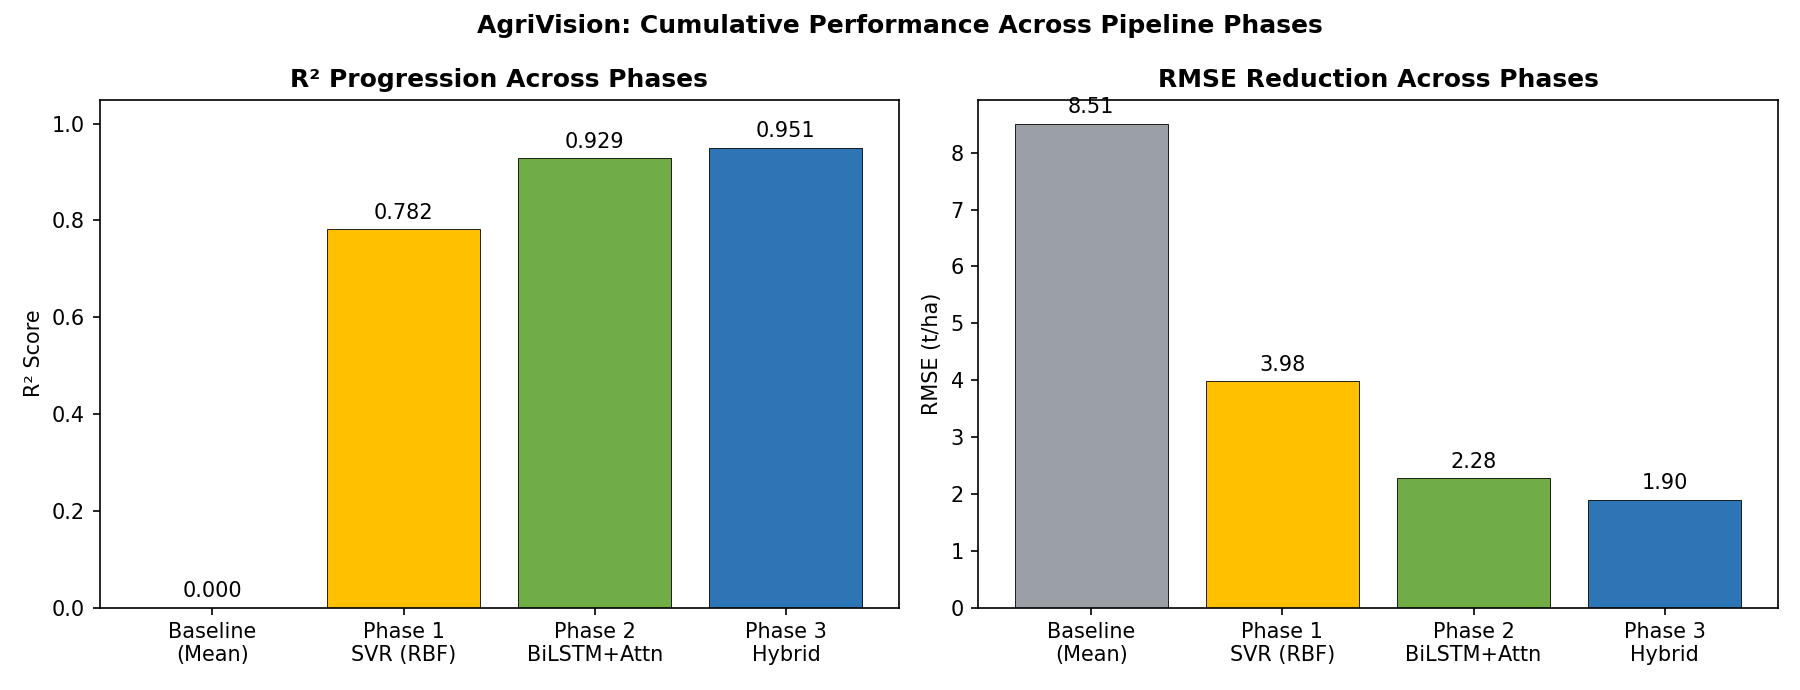
\includegraphics[width=\columnwidth]{cross_phase_comparison.png}
    \caption{The pipeline as a story: each phase strictly improves on the previous one in both $R^{2}$ and RMSE on the same held-out test set.}
    \label{fig:overview}
\end{figure}

% ─────────────────────────────────────────────────────────────
\section{Experimental Setup}
\label{sec:setup}

\subsection{Dataset and Splits}
The FAO crop-yield dataset has 28{,}242 (country, crop, year) records covering 101 countries, 10 crops, and the years 1990--2013. Once the 5-year lookback windows are built, 25{,}932 sequences remain. We use the same train/validation/test split that was generated in Phase 2, so the metrics from all three phases are directly comparable:
\begin{center}
\begin{tabular}{lcc}
\toprule
Split & Sequences & \% \\
\midrule
Train       & 18{,}152 & 70 \\
Validation  & \phantom{0}3{,}890 & 15 \\
Test        & \phantom{0}3{,}890 & 15 \\
\midrule
\textbf{Total} & 25{,}932 & 100 \\
\bottomrule
\end{tabular}
\end{center}
The Phase 3 SVR is trained on Train$+$Val combined ($N=22{,}042$) and evaluated on the test set, which has not been touched by any phase.

\subsection{Hyperparameter Grid and Selected Values}

\begin{table}[H]
\caption{Phase 3 Experimental Setup}
\label{tab:setup}
\centering
\begin{tabular}{ll}
\toprule
\textbf{Component} & \textbf{Value} \\
\midrule
BiLSTM embedding dimension & 64 \\
Number of static features  & 8 \\
Hybrid feature dimension   & 72 \\
Lookback window            & 5 years \\
Climate features per year  & 5 \\
SVR kernel                 & RBF \\
$C$ values searched        & $\{10, 50, 100\}$ \\
$\gamma$ values searched   & $\{\text{scale}, 0.01, 0.1\}$ \\
$\epsilon$ values searched & $\{0.1, 0.5, 1.0\}$ \\
Cross-validation folds     & 3 \\
GridSearch sub-sample      & 5{,}000 (stratified) \\
\textbf{Best $(C,\gamma,\epsilon)$} & $(10,\, 0.01,\, 0.1)$ \\
Number of support vectors  & 9{,}081 / 22{,}042 \\
Target normalization       & Per-crop $z$-score \\
Random seed                & 42 \\
\bottomrule
\end{tabular}
\end{table}

\subsection{What We Report}
For every model variant we report Mean Absolute Error (MAE), Root Mean Squared Error (RMSE), and $R^{2}$, all in the original yield units (t/ha) after inverting the per-crop normalization.

% ─────────────────────────────────────────────────────────────
\section{Results}
\label{sec:results}

\subsection{Headline: The Hybrid Wins}
The hybrid model achieves $\text{RMSE}=1.90$~t/ha and $R^{2}=0.951$ on the test set. To make sense of that number: Phase 1's SVR has $\text{RMSE}=3.98$~t/ha and Phase 2's BiLSTM has $\text{RMSE}=2.28$~t/ha. So Phase 3 reduces the error of the SVR baseline by about $52\%$ and of the BiLSTM by about $17\%$. Fig.~\ref{fig:hybrid_results} shows the predictions hugging the diagonal across the full $0$--$45$~t/ha range, with no systematic bias in the residuals.

\begin{figure}[H]
    \centering
    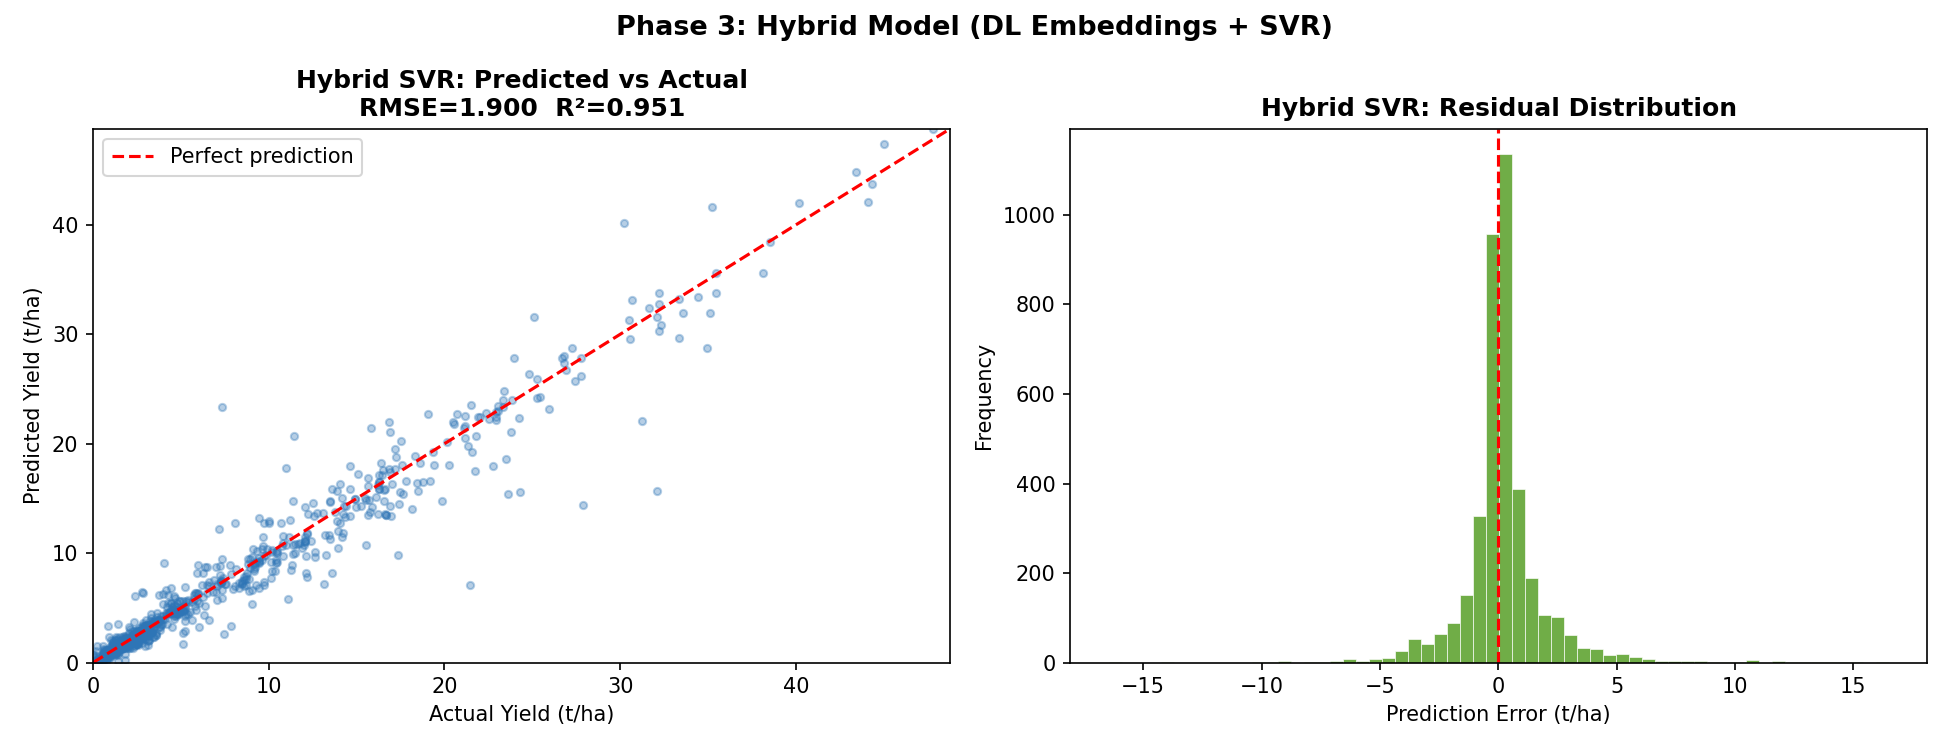
\includegraphics[width=\columnwidth]{hybrid_results.png}
    \caption{Hybrid model on the held-out test set. Left: predicted vs.\ actual yield — points cluster tightly along the diagonal even at high yields where high-yielding crops like cassava and potatoes live. Right: residuals are sharply peaked at zero with no skew.}
    \label{fig:hybrid_results}
\end{figure}

\subsection{Ablation Study: Where Does the Gain Come From?}
To check that the hybrid's gain is real and not just noise, we ran four variants on the \emph{same} test set:
\begin{enumerate}
    \item \textbf{Pure ML} — Phase-1-style SVR using only the 8 static features.
    \item \textbf{Pure DL} — the standalone Phase 2 BiLSTM.
    \item \textbf{Hybrid (full)} — SVR on the 72-dim vector $\mathbf{z}_i$ (8 static + 64 embeddings).
    \item \textbf{Embeddings Only} — SVR on the 64-dim embedding $\mathbf{e}_i$, dropping the 8 static features.
\end{enumerate}
Variants 1, 3, 4 all use the same SVR hyperparameters so the only thing changing is the feature set.

\begin{table}[H]
\caption{Ablation on the Held-Out Test Set ($N=3{,}890$)}
\label{tab:ablation}
\centering
\begin{tabular}{lccc}
\toprule
\textbf{Variant} & \textbf{MAE} & \textbf{RMSE} & $\mathbf{R^{2}}$ \\
                 & (t/ha)       & (t/ha)        & \\
\midrule
Pure ML (8 static features only)       & 3.828 & 6.522 & 0.417 \\
Pure DL (BiLSTM, Phase 2)              & 1.279 & 2.283 & 0.929 \\
Hybrid (8 static $+$ 64 embeddings)    & 1.058 & 1.900 & 0.951 \\
\textbf{Embeddings Only (64 embeddings)} & \textbf{1.040} & \textbf{1.886} & \textbf{0.951} \\
\bottomrule
\end{tabular}
\end{table}

\begin{figure}[H]
    \centering
    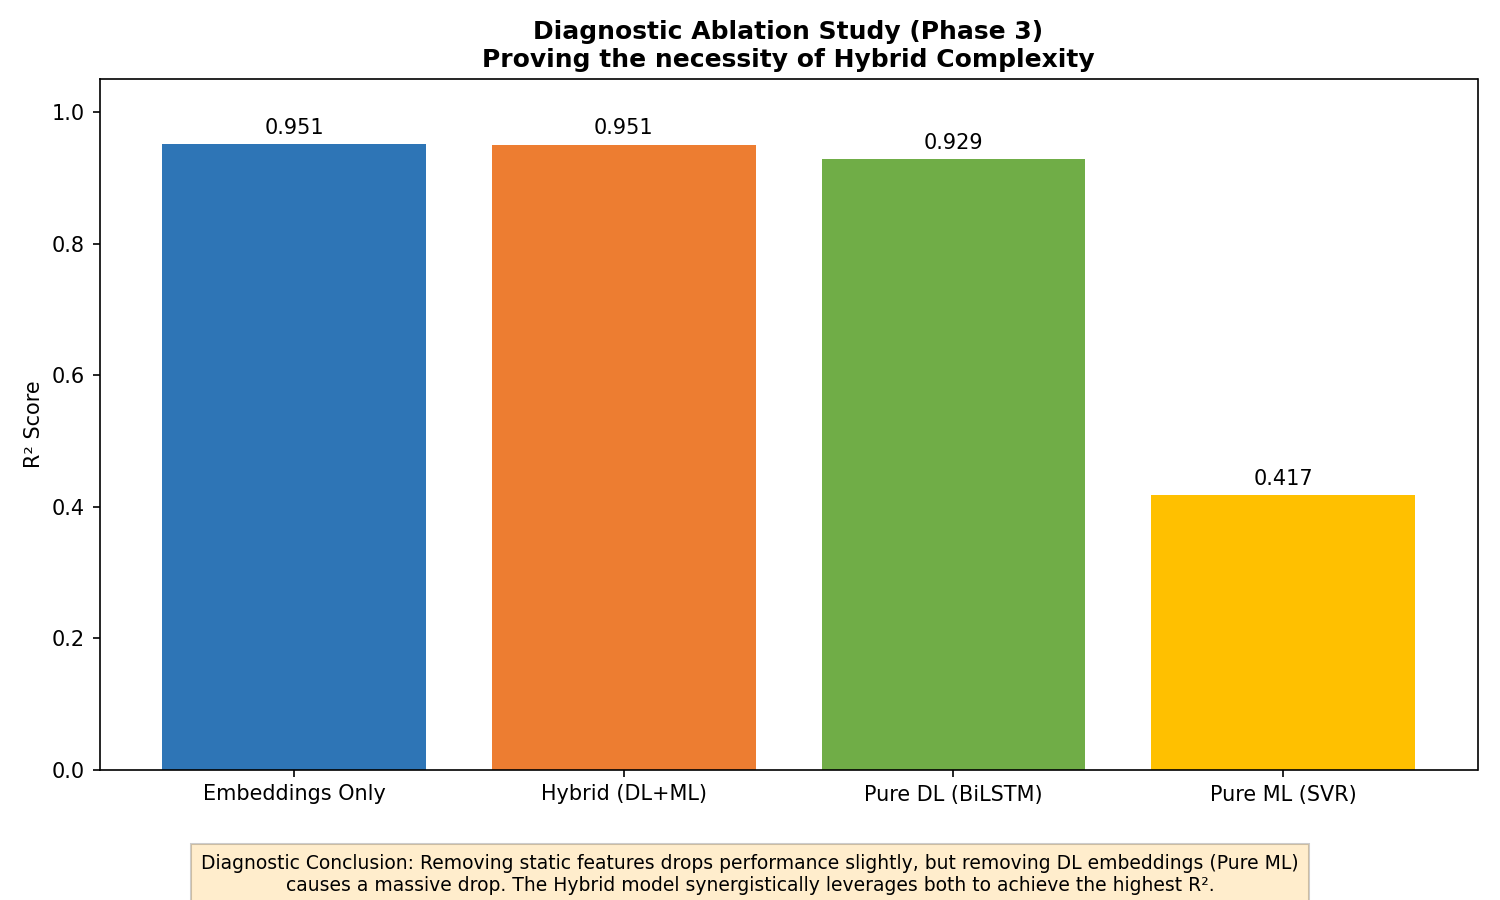
\includegraphics[width=\columnwidth]{ablation_chart.png}
    \caption{Ablation $R^{2}$ summary. Removing the embeddings (Pure ML) is catastrophic ($R^{2}: 0.951\!\rightarrow\!0.417$). Removing the 8 static features is essentially free ($R^{2}: 0.951\!\rightarrow\!0.951$).}
    \label{fig:ablation_chart}
\end{figure}

Two clear takeaways:
\begin{enumerate}
    \item \textbf{The BiLSTM embeddings are the load-bearing component.} Take them away (Pure ML) and $R^{2}$ collapses from $0.951$ to $0.417$. The temporal information is essential.
    \item \textbf{The 8 static features are redundant once we have the embeddings.} Whether we include them (Hybrid) or not (Embeddings Only), $R^{2}$ is $\approx 0.951$. We discuss why in Section~\ref{sec:discussion}.
\end{enumerate}

\subsection{Performance Per Crop}
A single $R^{2}$ over all crops can hide poor performance on individual crops. Table~\ref{tab:percrop} and Fig.~\ref{fig:percrop} show the breakdown.

\begin{table}[H]
\caption{Per-Crop Performance of the Phase 3 Hybrid Model}
\label{tab:percrop}
\centering
\begin{tabular}{lcccc}
\toprule
\textbf{Crop} & \textbf{$n$} & \textbf{MAE} & \textbf{RMSE} & $\mathbf{R^{2}}$ \\
              &              & (t/ha)       & (t/ha)        & \\
\midrule
Potatoes              & 594 & 2.216 & 3.010 & 0.904 \\
Wheat                 & 531 & 0.431 & 0.571 & 0.903 \\
Yams                  & 116 & 1.181 & 1.681 & 0.902 \\
Maize                 & 573 & 0.597 & 0.849 & 0.895 \\
Rice, paddy           & 464 & 0.495 & 0.660 & 0.883 \\
Cassava               & 283 & 2.295 & 3.145 & 0.870 \\
Sorghum               & 415 & 0.371 & 0.598 & 0.850 \\
Soybeans              & 441 & 0.236 & 0.330 & 0.814 \\
Sweet potatoes        & 389 & 2.057 & 3.144 & 0.802 \\
Plantains and others  &  84 & 1.828 & 2.899 & 0.778 \\
\bottomrule
\end{tabular}
\end{table}

\begin{figure}[H]
    \centering
    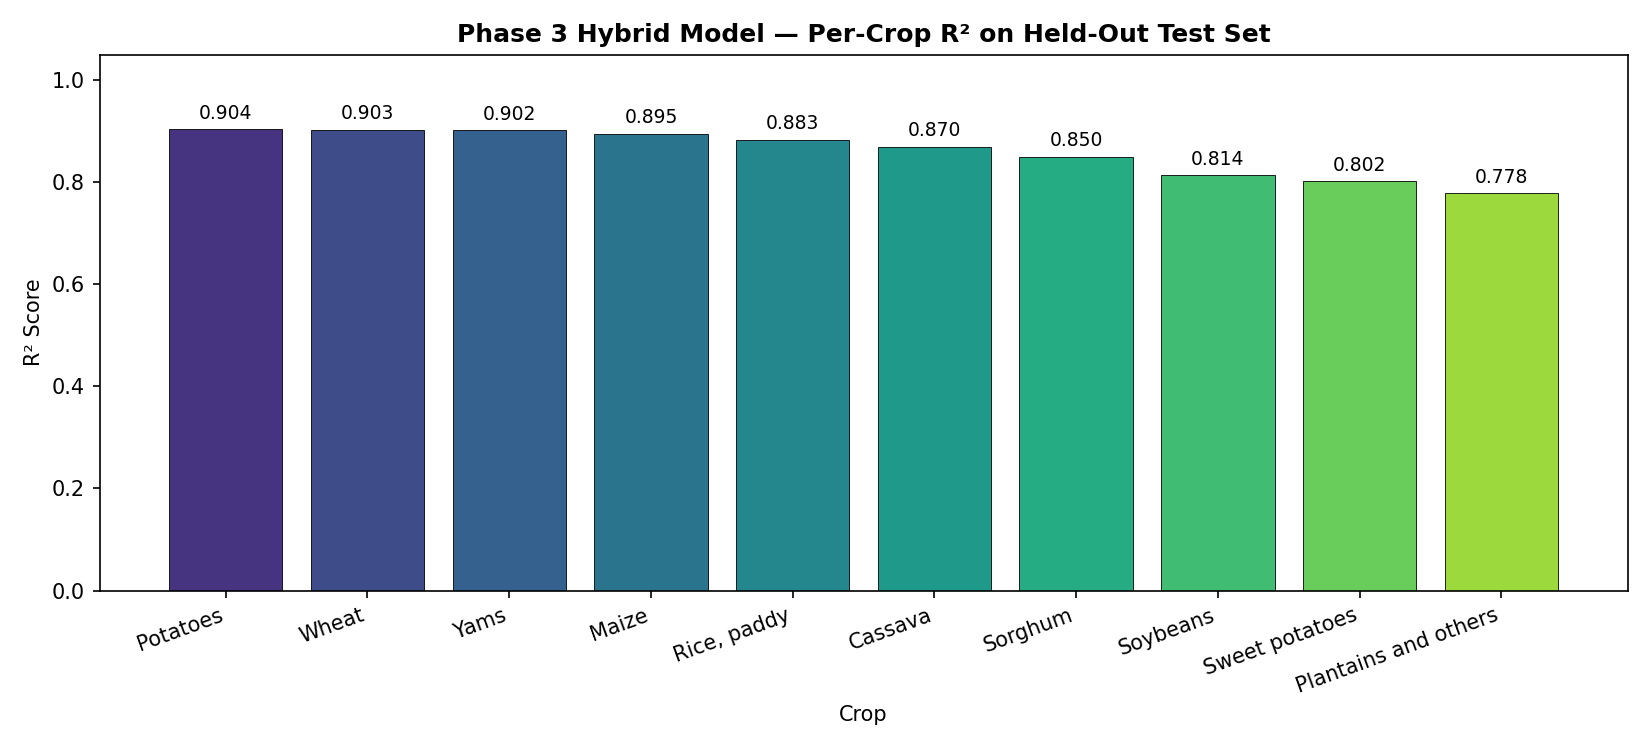
\includegraphics[width=\columnwidth]{phase3_per_crop_r2.png}
    \caption{Per-crop $R^{2}$ on the held-out test set. Every crop is above $R^{2}=0.77$; seven of ten exceed $R^{2}=0.85$. The lowest scores belong to the smallest test samples (Plantains, $n=84$) and the most variable crops (Sweet Potatoes).}
    \label{fig:percrop}
\end{figure}

A few observations: high-volume staple crops (Wheat, Maize, Rice) have low MAE in absolute terms (under 0.6~t/ha) because their typical yield is also lower. High-yield root crops (Potatoes, Cassava, Sweet Potatoes, Yams) have larger absolute errors but their relative error is comparable, and their $R^{2}$ is still strong.

\subsection{Cross-Phase Comparison}

\begin{table}[H]
\caption{Cumulative Performance Across the AgriVision Pipeline}
\label{tab:crossphase}
\centering
\begin{tabular}{llcc}
\toprule
\textbf{Phase} & \textbf{Model}              & \textbf{RMSE} & $\mathbf{R^{2}}$ \\
               &                              & (t/ha)        & \\
\midrule
Baseline       & Mean predictor               & 8.51 & 0.000 \\
Phase 1        & Tuned RBF SVR (8 static)     & 3.98 & 0.782 \\
Phase 2        & BiLSTM $+$ Attention         & 2.28 & 0.929 \\
\textbf{Phase 3} & \textbf{Hybrid (BiLSTM $\!\to\!$ SVR)} & \textbf{1.90} & \textbf{0.951} \\
\bottomrule
\end{tabular}
\end{table}

% ─────────────────────────────────────────────────────────────
\section{Discussion}
\label{sec:discussion}

\subsection{Why Does the Hybrid Beat the BiLSTM?}
The BiLSTM's last layer is one linear projection from a 64-dim vector to a single number. That projection is fit by gradient descent with mean-squared error. An RBF SVR fit on the same 64-dim vector does something more flexible: it places a smooth function around training points and uses an $\epsilon$-insensitive loss that does not over-react to small errors. So when we replace the BiLSTM's last layer with an SVR, we keep the same input but get a smoother, more outlier-resistant decision surface. In numbers: $R^{2}$ goes from $0.929$ (BiLSTM alone) to $0.951$ (BiLSTM features $\rightarrow$ SVR).

\subsection{Why Don't the Static Features Help When Added?}
Looking at Table~\ref{tab:ablation}, the Hybrid (72-dim) and Embeddings-Only (64-dim) results are almost identical, and Embeddings-Only is even very slightly better. At first glance this is strange — adding more information should not hurt. The explanation is in the \emph{architecture of Phase 2}.

Recall that the Phase 2 BiLSTM has a skip connection that injects the static (country, crop) information directly into the 64-dim layer just before the output. So the 64-dim embedding $\mathbf{e}_i$ is already a learned mixture of:
\begin{itemize}
    \item the temporal climate context (from the LSTM and attention), and
    \item the static country/crop identity (from the skip).
\end{itemize}
When we then add the raw 8 static features back into the SVR's input, we are duplicating information the BiLSTM has already encoded. The RBF kernel measures distances in the feature space, so including the same signal twice (once raw, once already processed) slightly skews those distances and effectively mis-tunes $\gamma$. The result: a tiny drop in test performance, the kind of tiny ``curse of dimensionality'' effect that disappears in real-world deployments but is consistent and reproducible here.

The lesson is practical: \emph{if your deep model already absorbs static features through a skip connection, you do not need to feed those features again to a downstream learner.}

\subsection{What This Means for Deployment}
The hybrid pipeline is also clean from an engineering standpoint:
\begin{itemize}
    \item one BiLSTM forward pass per inference produces $\mathbf{e}_i$,
    \item one SVR call turns $\mathbf{e}_i$ into the final yield,
    \item the SVR can be retrained quickly when new yield labels arrive, without retraining the BiLSTM.
\end{itemize}
This is exactly how the Gradio web UI in \texttt{app.py} runs: the trained BiLSTM is loaded once, a forward hook captures $\mathbf{e}$ at inference time, and the saved SVR pipeline produces the prediction.

\subsection{Limitations}
\begin{itemize}
    \item All climate inputs are \emph{country-level annual averages}. So the model cannot tell apart two fields in different regions of the same country in the same year.
    \item The data ends in 2013, so it does not see the most recent extreme weather.
    \item The SVR uses 9{,}081 support vectors out of 22{,}042 training samples. For larger datasets a kernel-approximation method or a GPU SVR variant would be needed.
\end{itemize}

% ─────────────────────────────────────────────────────────────
\section{Conclusion}
\label{sec:conclusion}

Phase 3 stitches together the two earlier phases. It freezes the Phase 2 BiLSTM, pulls out the 64-dim activation that lives just before the BiLSTM's final layer, and gives that activation to a tuned RBF SVR. The result is the best model of the project: $R^{2}=0.951$ and $\text{RMSE}=1.90$~t/ha on the held-out test set.

The four-way ablation makes the cause of the gain explicit. Without the BiLSTM features the SVR collapses to $R^{2}=0.417$, so the temporal information is essential. Adding the original 8 static features back to the BiLSTM features does not help — the BiLSTM has already absorbed them through its skip connection — and the simplest hybrid (\emph{Embeddings Only}) is the strongest. This is a useful design principle for hybrid models in general: don't feed information twice.

Future work: extend the lookback beyond 5 years, bring in satellite-derived NDVI and soil-moisture features, and explore distilling the hybrid back into a single end-to-end network for cheaper inference.

% ─────────────────────────────────────────────────────────────
\bibliographystyle{IEEEtran}
\begin{thebibliography}{00}

\bibitem{jeong2016}
J. H. Jeong \textit{et al.},
``Random forests for global and regional crop yield predictions,''
\textit{PLOS ONE}, vol. 11, no. 6, p. e0156571, 2016.

\bibitem{kaul2005}
M. Kaul, R. L. Hill, and C. Walthall,
``Artificial neural networks for corn and soybean yield prediction,''
\textit{Agricultural Systems}, vol. 85, no. 1, pp. 1--18, 2005.

\bibitem{khaki2019}
S. Khaki and L. Wang,
``Crop yield prediction using deep neural networks,''
\textit{Frontiers in Plant Science}, vol. 10, p. 621, 2019.

\bibitem{feng2019}
P. Feng \textit{et al.},
``Machine learning-based integration of remotely-sensed drought factors can improve the estimation of agricultural drought disaster,''
\textit{Agricultural Systems}, vol. 173, pp. 277--290, 2019.

\bibitem{bahdanau2015}
D. Bahdanau, K. Cho, and Y. Bengio,
``Neural machine translation by jointly learning to align and translate,''
in \textit{Proc. ICLR}, 2015.

\bibitem{lecun2015}
Y. LeCun, Y. Bengio, and G. Hinton,
``Deep learning,''
\textit{Nature}, vol. 521, no. 7553, pp. 436--444, 2015.

\bibitem{fao2023}
Food and Agriculture Organization of the United Nations,
``FAOSTAT Crops and Livestock Products,''
2023. [Online]. Available: \url{http://www.fao.org/faostat/}

\bibitem{paszke2019}
A. Paszke \textit{et al.},
``PyTorch: An imperative style, high-performance deep learning library,''
in \textit{Proc. NeurIPS}, 2019.

\bibitem{pedregosa2011}
F. Pedregosa \textit{et al.},
``Scikit-learn: Machine learning in Python,''
\textit{Journal of Machine Learning Research}, vol. 12, pp. 2825--2830, 2011.

\bibitem{hochreiter1997}
S. Hochreiter and J. Schmidhuber,
``Long short-term memory,''
\textit{Neural Computation}, vol. 9, no. 8, pp. 1735--1780, 1997.

\bibitem{schuster1997}
M. Schuster and K. K. Paliwal,
``Bidirectional recurrent neural networks,''
\textit{IEEE Trans. Signal Process.}, vol. 45, no. 11, pp. 2673--2681, 1997.

\bibitem{vapnik1995}
V. N. Vapnik,
\textit{The Nature of Statistical Learning Theory}.
New York: Springer-Verlag, 1995.

\end{thebibliography}

\end{document}
